\documentclass[11pt]{article}
\usepackage{graphicx}
\usepackage[export]{adjustbox}
\usepackage{float}
\usepackage{amsmath}
\usepackage{siunitx}
\title{Three Phase Circuits}
\date{2018\\ March}
\author{Nail Tosun - 2094563 -Section 5\\ Electric and Electronic Engineering Departmant, METU}
\begin{document}
\maketitle
\section*{Examples}
\subsection*{Homework 4}

1)

\begin{figure}[H]
  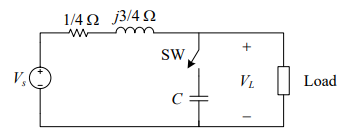
\includegraphics[scale=1, center]{hw5q1}
  \caption{Question}
  \label{fig:zero}
\end{figure}
$V_{L}6\sqrt{5}$ and $pf=\frac{1}{\sqrt{5}}$ obtainin phasor diagram. Related phasor diagram is;
\begin{figure}[H]
  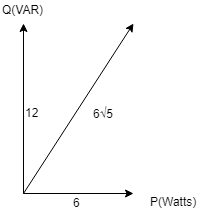
\includegraphics[scale=0.6, center]{phasor1}
  \caption{Phasor diagram of load}
  \label{fig:zero}
\end{figure}
  Since total reactive power 24 VAR and load reactive power 12 VAR; reactive power on $j\frac{3}{4}$ is 12 VAR.
 \[12=I_A^2X_{j0.75}\]
 \[I_A=4A\]
 \[P_{\frac{1}{4}\si{\ohm}}=4W\]
 \[S_{total}=26VA=V_{RMS}I_{RMS}\]
 \[V_{S_{RMS}}=6.5V\]
 \[S_L=6\sqrt{5}VA=V_{RMS}I_{RMS}\]
 \[V_{S_{RMS}}=\frac{3\sqrt{5}}{2}\]
\begin{figure}[H]
  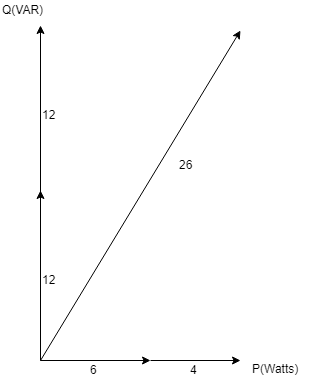
\includegraphics[scale=0.6, center]{overallphasor}
  \caption{Overall phasor diagram}
  \label{fig:zero}
\end{figure}
Then switch closed, since load voltage kept same load has same phasor diagram.
\[P=7W\]
1W comes from line resistor meaning that $I_A=4\>A$ then $Q_{j\frac{3}{4}}=3\> VAR$. There are infinite solution for each capacitor values. however for the sake of calculation i set $Q_c=15\>VAR$
\begin{figure}[H]
  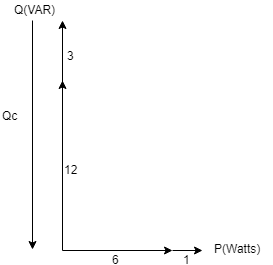
\includegraphics[scale=0.6, center]{new-phasor}
  \caption{Updated phasor diagram}
  \label{fig:zero}
\end{figure}
\[Q_c=-15=\frac{45}{4X_c}\]
\[X_c=-j\frac{3}{4}\]
\[B_c=\frac{4}{3}S\]
\end{document}